

\chapter{The Memory System}
\label{sec:memory}


\section{Caches}

Each cache structure consists of the cache storage (tag and data) and multiple
queues. Figure~\ref{fig:cache} shows the overall structure of a cache in \SIM.
There are two flows: 1) cache access flow: from a processor or upper level
cache miss, to access the cache and 2) cache fill flow: in case of a cache
miss, data is supplied from the lower level cache or DRAM.
Section~\ref{sec:queue} details all queues and Section~\ref{sec:cache-flow}
lists the flows through the queues and the cache.

\begin{figure*}[htb]
\centering
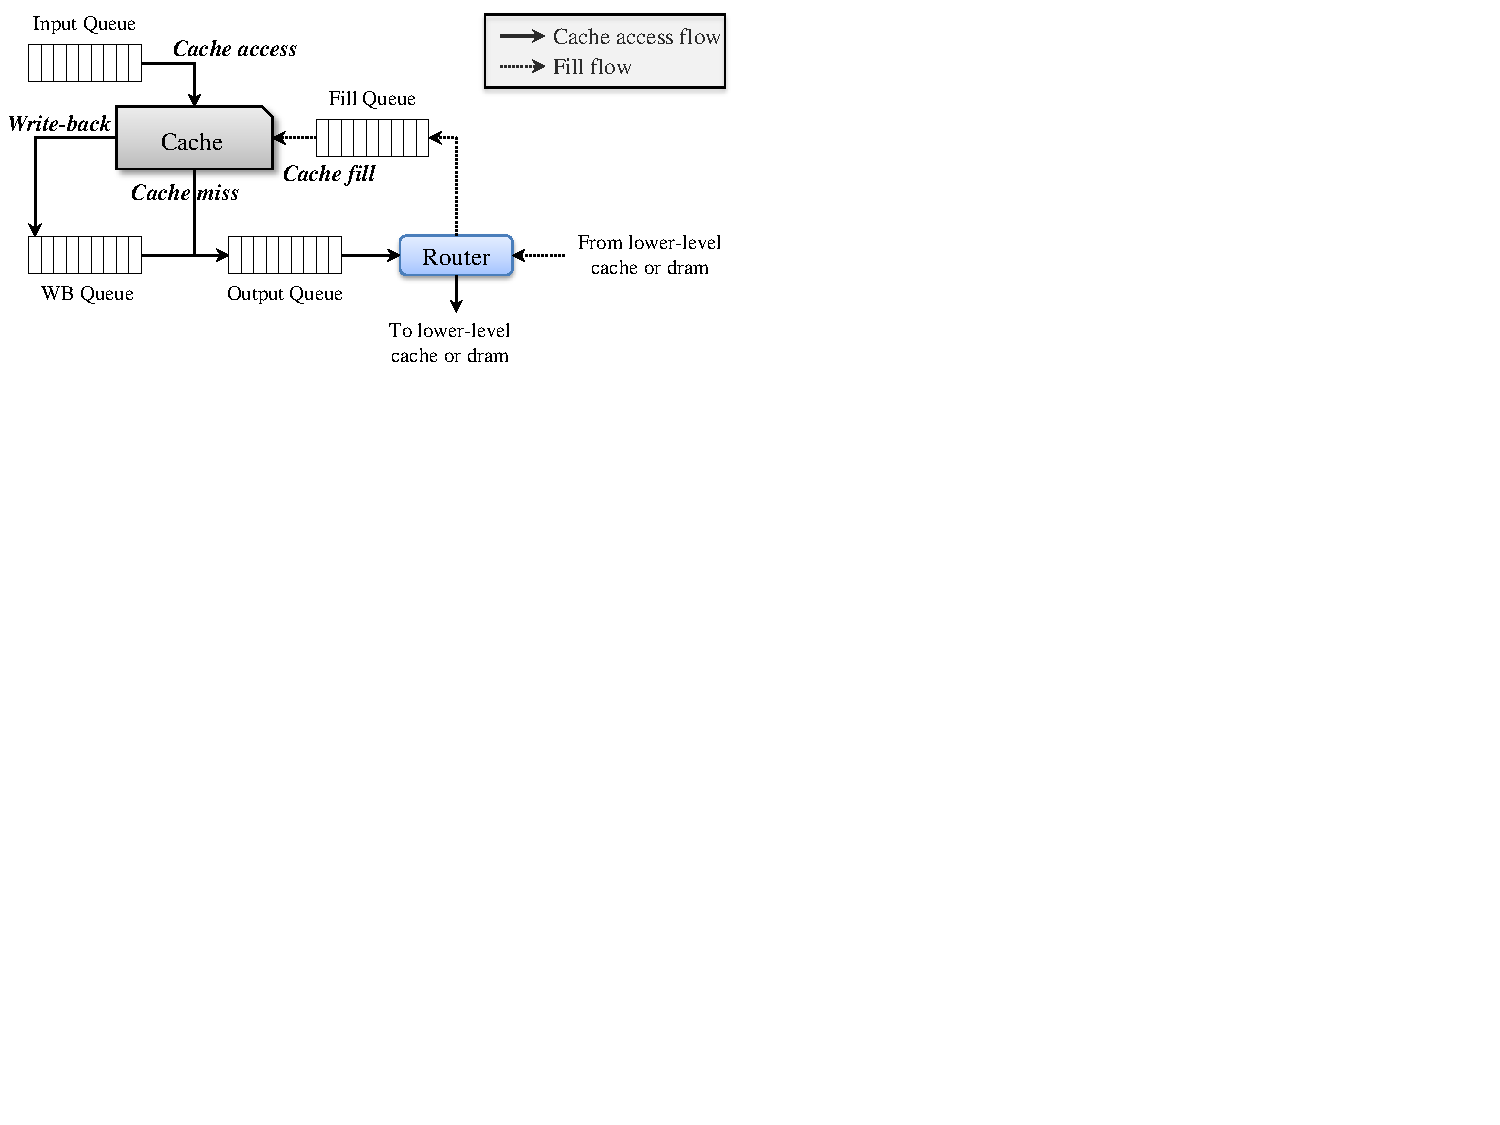
\includegraphics{figs/cache}
\caption{The cache structure.}
\label{fig:cache}
\end{figure*}


\subsection{The Queues}
\label{sec:queue}

All cache accesses flow from one queue to another.

\begin{itemize}
  \item input queue - requests forwarded to this cache due to upper-level cache misses are inserted into this queue.

  \item output queue - requests that miss in this cache are inserted into the
  output queue to be forwarded to a lower-level cache . If no lower-level cache
  is available, then requests are forwarded to DRAM.

  \item write-back queue - \SIM models write-back caches. When a dirty cache
  line is evicted, the line must be written back into the next level cache (or
      DRAM). All write-back requests are initially inserted into the write-back
  queue.

  \item fill queue - data returned from the next level cache or DRAM is
  inserted into the fill queue before updating the cache.

%  \item coherence queue - this queue is intended for handling coherence
%  traffic, but this is currently not modeled
  
\end{itemize}


\subsection{The Flows}
\label{sec:cache-flow}

\begin{itemize}

  \item Upper-level cache to input queue : forwarding of upper-level cache misses

  \item Upper-level cache to fill queue : forwarding of upper-level write-back requests

  \item input queue to cache : accessing the cache

  \item cache to output queue : cache miss, access lower-level cache

  \item cache to write-back queue : generating write-back requests

  \item write-back queue to output queue : write-back request, access the
  lower-level cache

  \item output queue to the router : access the lower-level cache
  through the on-chip interconnection network

  \item router to the fill queue : the data from the lower-level cache
  or DRAM

\end{itemize}


\section{The Hierarchy}
\label{sec:memhierarchy}

\SIM is very flexible in its support for different memory
hierarchies. Each level in the cache hierarchy can be configured
independently of other levels (see Section~\ref{sec:knob:cache}).
Figure~\ref{fig:memory} shows the base memory hierarchy without DRAM
memory.

\begin{figure*}[htb]
\centering
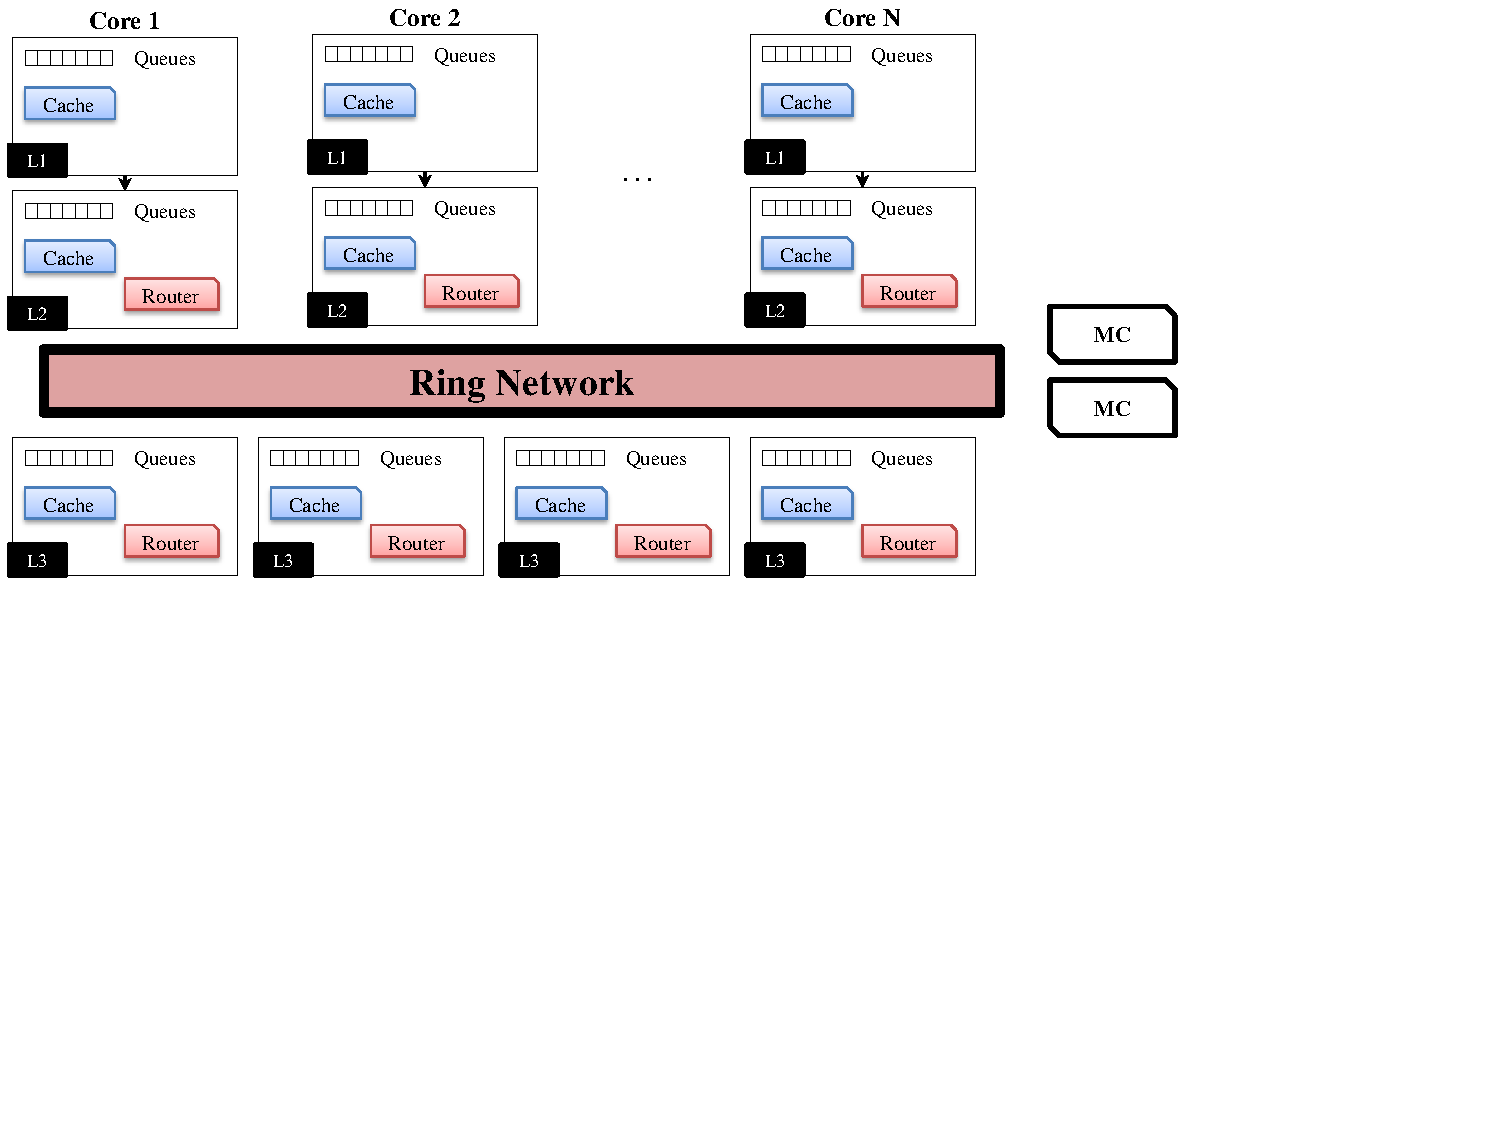
\includegraphics[width=6.5in]{figs/memory}
\caption{The memory system in \SIM.}
\label{fig:memory}
\end{figure*}


\begin{itemize} \item There are three levels (L1, L2, and L3) of caches in the
\SIM , the L2 cache can be disabled if needed by some configurations.

  \item All the caches and memory controllers can be connected via an
    on-chip interconnection network (currently, the default topology
    is ring), if the configuration allows.

  \item L1 and L2 caches are always private to each core.

  \item The local router within a cache structure is enabled only when
  necessary.

  \item L3 cache is unified (shared by all cores), but sub banked. In
    other words, address regions are statically partitioned and each
    tile is responsible for sub regions. Each cache tile has multiple
    banks as well.

\end{itemize}


Figure~\ref{fig:level2cache} shows how to configure a 2-level cache hierarchy.
Even though there are 3-levels of cache, the L2 cache is disabled and only its
router is used by the L1 cache to access the interconnection network. Since
there is no additional latency between L1 and L2 when the L2 is disabled, we
can flexibly configure 2-level cache hierarchies.


\begin{figure*}[htb]
\centering
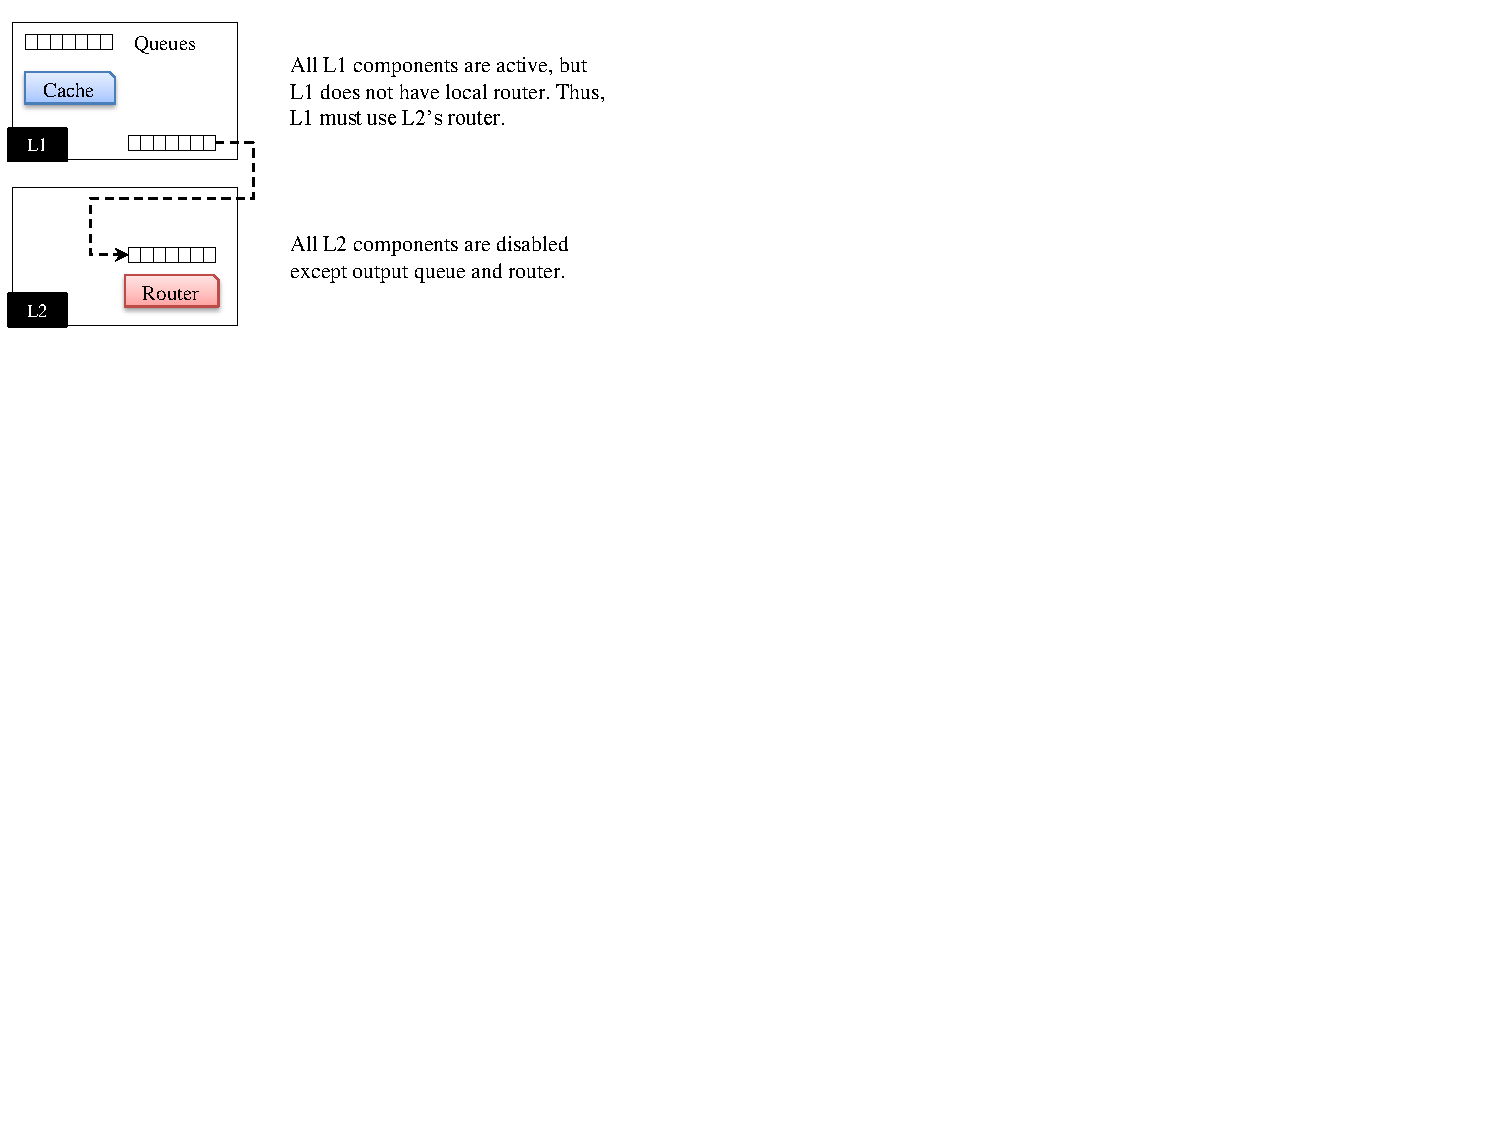
\includegraphics{figs/level2cache}
\caption{2-Level cache hierarchy.}
\label{fig:level2cache}
\end{figure*}


\section{Configuring the Cache Hierarchy} 

The cache hierarchy can be configured by 1) setting the link between different
cache levels, 2) disabling cache levels and 3) enabling/disabling routers. The
following code is used in \SIM for cache initialization.

\begin{Verbatim}
void dcu_c::init(
  int next_id, // next level cache id
  int prev_id, // previous level cache id
  bool done, 
  bool coupled_up, // direct link with upper level cache
  bool coupled_down, // direct link with lower level cache
  bool disable, // disable cache
  bool has_router // router
);
\end{Verbatim}

\begin{description}
  \item[Enabling/disabling router] When \textsf{has\_router} is set to \textit{false},
  the cache cannot directly access to the on-chip
  interconnection. Instead, it has to go through lower-level cache's
  interface. Therefore, \textsf{coupled\_down} must set
  to \textit{true} and appropriate \textsf{next\_id} must be set. In
  this way, the output queue of the cache is connected directly to the
  input queue of the next level (lower) cache.

  \item[Disabling cache levels] When \textsf{disable} is set to \textit{true},
  the cache is disabled. When a request is inserted into the input queue of a
  disabled cache, the request will be directly inserted into the output queue
  of the cache. This feature has been used for modeling 2-level cache
  hierarchies. As Figure~\ref{fig:level2cache} shows, L1 and L3 caches are
  active, but L2 cache is disabled. However, since the L1 cache does not have a
  router, it needs to use the router of the L2 cache. Therefore,
  \textsf{has\_router} must be set to \textit{true} for the L2 cache.

  \item[Links] As mentioned in the Section~\ref{sec:memhierarchy}, the
  L1 and L2 caches are always private to a core. All L1 misses
  should go through the L2 cache without accessing the interconnection
  network. To this end, a direct link must be set between the L1 and
  L2 caches. Therefore, \textsf{coupled\_down} and \textsf{next\_id}
  must be set for the L1 cache and \textsf{coupled\_up}
  and \textsf{prev\_id} must be set for the L2 cache. Note that the
  link is always bi-directional.

\end{description}

\subsection{Configuring Different Cache Hierarchies with \SIM}


\begin{itemize}
\ignore{
  \item Intel Core~\cite{core2duo} microarchitecture has two-level of
  caches. The last-level cache might be tiled, but if the L2 cache
  tries to access the closest the L3 tile, it does not have to access
  through the interconnection. All communications will be made through
  the direct link. However, if the L2 cache accesses the remote L3
  tile, it goes through the interconnection. Note that the number of
  cores (L1 and L2 caches) and the number of the L3 tiles must be the
  same.

  \smallskip
  \begin{lstlisting}
  // class l2_coupled_local_c
  \end{lstlisting}
  \smallskip
}

  \item Intel Nehalem~\cite{nehalem} and Sandy
    Bridge~\cite{sandybridge} microarchitectures have three-levels of
    caches. The last-level cache is tiled and to access the closest L3
    tile, a L2 cache does not have to go through the interconnection,
    it can access the L3 tile directly. However, if a L2 cache
    accesses a remote L3 tile, it goes through the interconnection.
    Note that the number of cores (L1 and L2 caches) and the number of
    the L3 tiles must be the same in this configuration.

\begin{Verbatim}
// class l3_coupled_network_c
for (int ii = 0; ii < m_num_core; ++ii) {
  // next_id, prev_id, done, coupled_up, coupled_down, disable, router
  m_l1_cache[ii]->init(ii, -1, false, false, TRUE, false, false);
  m_l2_cache[ii]->init(ii, ii, true,  TRUE,  TRUE, false, TRUE);
  m_l3_cache[ii]->init(-1, ii, false, TRUE,  false,false, TRUE);
}
\end{Verbatim}

  \item NVIDIA G80~\cite{g80} architecture does not have
  hardware-managed caches. Thus, all three levels are connected each
  other and disabled. Only the L3 cache has a router to access the DRAM.

  \begin{Verbatim}
  // class no_cache_c
  for (int ii = 0; ii < m_num_core; ++ii) {
    // next_id, prev_id, done, coupled_up, coupled_down, disable, router
    m_l1_cache[ii]->init(ii, -1, false, false, TRUE,  TRUE, false);
    m_l2_cache[ii]->init(ii, ii, true,  TRUE,  TRUE,  TRUE, false);
    m_l3_cache[ii]->init(-1, ii, false, TRUE,  false, TRUE, TRUE);
  }
  \end{Verbatim}

  \item NVIDIA Fermi~\cite{fermi} architecture has private L1 caches and a
  unified L2 cache shared by all cores. The L1 and L2 caches are linked. The L2
  cache is been disabled, but has is router enabled. The L3 is not linked with
  others (it is connected via the interconnect), but it is enabled and has a
  router.

  \begin{Verbatim}
  // class l2_decoupled_network_c
  // next_id, prev_id, done, coupled_up, coupled_down, disable, router
  for (int ii = 0; ii < m_num_core; ++ii) {
    m_l1_cache[ii]->init(ii, -1, false, false, TRUE,  false, false);
    m_l2_cache[ii]->init(-1, ii, true,  TRUE,  false, true,  true);
  }

  for (int ii = 0; ii < m_num_l3; ++ii) {
    // next_id, prev_id, done, coupled_up, coupled_down, disable, router
    m_l3_cache[ii]->init(-1, -1, false, false, false, false, true);
  }
  \end{Verbatim}
  
  \item In a general 2-D Topology (Mesh, Torus), it is assumed that each core
  has private L1 and L2 caches, but access to the L3 cache must be 
  through the interconnection network. The L1 and L2 caches are both enabled
  and linked, but only the L2 cache has a router. The L3 cache is not linked
  with other caches and the communication is made through the interconnection
  network.

  \begin{Verbatim}
  // class l3_decoupled_network_c
  // next_id, prev_id, done, coupled_up, coupled_down, disable, router
  for (int ii = 0; ii < m_num_core; ++ii) {
    m_l1_cache[ii]->init(ii, -1, false, false, TRUE,  false, false);
    m_l2_cache[ii]->init(-1, ii, true,  TRUE,  false, false, TRUE);
  }

  for (int ii = 0; ii < m_num_l3; ++ii) {
    // next_id, prev_id, done, coupled_up, coupled_down, disable, router
    m_l3_cache[ii]->init(-1, -1, false, false, false, false, TRUE);
  }
  \end{Verbatim}
\end{itemize}


%%%%%%%%%%%%%%%%%%%%%%%%%%%%%%%%%%%%%%%%%%%%%%%%%%%%%%%%%%%%%%%%%%%%%%%%
\section{DRAM Module} 
\label{sec:dram}
%%%%%%%%%%%%%%%%%%%%%%%%%%%%%%%%%%%%%%%%%%%%%%%%%%%%%%%%%%%%%%%%%%%%%%%%


\SIM also models detailed memory controllers which consider DRAM
timing constraints and bandwidth specifications when scheduling
requests.  Section~\ref{sec:param-dram} describes how to configure
DRAM parameters.


%%%%%%%%%%%%%%%%%%%%%%%%%%%%%%%%%%%%%%%%%%%%%%%%%%%%%%%%%%%%%%%%%%%%%%%%
\subsection{DRAM Timing Constraints}
%%%%%%%%%%%%%%%%%%%%%%%%%%%%%%%%%%%%%%%%%%%%%%%%%%%%%%%%%%%%%%%%%%%%%%%%

We model following three timing constrainsts of DRAM.

\vspace{0.2in}
\begin{footnotesize}
\begin{tabular}{llll}
\Verb+Precharge+     & \Verb+KNOB_DRAM_PRECHARGE+ & T$_{RP}$  & Row precharge time                  \\
\Verb+Activate+      & \Verb+KNOB_DRAM_ACTIVATE+  & T$_{RCD}$ & Row address to column address delay \\
\Verb+Column Access+ & \Verb+KNOB_DRAM_COLUMN+    & T$_{CL}$  & CAS latency                          \\
\end{tabular}
\end{footnotesize}


%%%%%%%%%%%%%%%%%%%%%%%%%%%%%%%%%%%%%%%%%%%%%%%%%%%%%%%%%%%%%%%%%%%%%%%%
\subsection{DRAM Bandwidth}
%%%%%%%%%%%%%%%%%%%%%%%%%%%%%%%%%%%%%%%%%%%%%%%%%%%%%%%%%%%%%%%%%%%%%%%%
aaa

\ignore{
\vspace{0.2in}
\begin{footnotesize}
\begin{tabular}{llll}
\Verb+DRAM Frequency+                        & \Verb+KNOB_DRAM_PRECHARGE+ & T$_{RP}$  & Row precharge time                  \\
\Verb+DRAM Data bus width+                   & \Verb+KNOB_DRAM_ACTIVATE+  & T$_{RCD}$ & Row address to column address delay \\
\Verb+Number of dram controllers+            & \Verb+KNOB_DRAM_COLUMN+    & T$_{CL}$  & CAS latency                         \\
\Verb+Number of dram channels Column Access+ & \Verb+KNOB_DRAM_COLUMN+    & T$_{CL}$  & CAS latency                         \\
\end{tabular}
\end{footnotesize}
}

\ignore{
max_bandwidth =dram_f requency�dram_bus_width�dram_num_mc�dram_num_channel
(2)
For example, the maximum bandwidth of a DRAM system with the above parameter values is
800 MHz (0.8 GHz)*4 Bytes*2 MCs*2 Channels = 12.8GB/s.
Currently, MacSim provides multiple DRAM scheduling policies: FCFS (First-Come-First-Serve) and FR-
FCFS (First-Ready First-Come-First-Serve).
}

%%%%%%%%%%%%%%%%%%%%%%%%%%%%%%%%%%%%%%%%%%%%%%%%%%%%%%%%%%%%%%%%%%%%%%%%
\subsection{The Structure of DRAM Controller}
%%%%%%%%%%%%%%%%%%%%%%%%%%%%%%%%%%%%%%%%%%%%%%%%%%%%%%%%%%%%%%%%%%%%%%%%

A DRAM controller consists of multiple banks and one or more channels.
Each bank has its own request buffer and request scheduler. The bank
scheduler picks a request to service based on the policy.

\begin{itemize}
  \item The bank scheduler picks a request based on the policy (FCFS,
    FRFCFS, ...) if no request is being served currently.

  \item The channel scheduler picks a request from command-ready banks
    usually based on the oldest request firs. Based on the command,
    appropriate timing constraint (precharge, activate, or column
    access) is enforced on the bank.

  \item Once the column access signal is sent, the data is prepared
  from the DRAM chip (load) or the data is sent to the DRAM chip
  (store). Among multiple data-ready banks, the channel scheduler
  picks a request based on the policy (oldest-first).

  \item When the data is ready/sent for a request, the data is
  supplied to the cache (load) or the request is completed (store).

  \item If there are memory requests with the same address, these
  requests are merged into one dram request. 

\end{itemize}



% LocalWords:  prev bool microarchitecture Nehalem num init NVIDIA FCFS FRFCFS
